\documentclass[11pt]{article}
\usepackage{fullpage}
\usepackage{fancyhdr}

\usepackage{amsmath}
\usepackage{amssymb}
\usepackage{url}

\usepackage{listings}
\usepackage{color}
\lstset{language=Python,
        basicstyle=\footnotesize\ttfamily,
        showspaces=false,
        showstringspaces=false,
        tabsize=2,
        breaklines=false,
        breakatwhitespace=true,
        identifierstyle=\ttfamily,
        keywordstyle=\color[rgb]{0,0,1},
        commentstyle=\color[rgb]{0.133,0.545,0.133},
        stringstyle=\color[rgb]{0.627,0.126,0.941},
    }

\usepackage[pdftex]{graphicx}

% header
\fancyhead{}
\fancyfoot{}
\fancyfoot[C]{\thepage}
\fancyhead[R]{Daniel Foreman-Mackey}
\fancyhead[L]{Statistical Natural Language Processing --- Homework 2}
\pagestyle{fancy}
\setlength{\headsep}{10pt}
\setlength{\headheight}{20pt}

% shortcuts
\newcommand{\Eq}[1]{Equation (\ref{eq:#1})}
\newcommand{\eq}[1]{Equation (\ref{eq:#1})}
\newcommand{\eqlabel}[1]{\label{eq:#1}}
\newcommand{\Fig}[1]{Figure \ref{fig:#1}}
\newcommand{\fig}[1]{Figure \ref{fig:#1}}
\newcommand{\figlabel}[1]{\label{fig:#1}}

\newcommand{\pr}[1]{\ensuremath{p\left (#1 \right )}}
\newcommand{\lk}[1]{\ensuremath{\mathcal{L} \left ( #1 \right )}}
\newcommand{\bvec}[1]{\ensuremath{\boldsymbol{#1}}}
\newcommand{\dd}{\ensuremath{\, \mathrm{d}}}
\newcommand{\normal}[2]{\ensuremath{\mathcal{N} \left ( #1; #2 \right ) }}
\newcommand{\T}{^\mathrm{T}}

\newcommand{\data}{\mathcal{D}}
\newcommand{\code}[1]{{\sffamily #1}}


\begin{document}

The goal of this project is to classify a noun into one of five categories
(\code{place}, \code{movie}, \code{drug}, \code{person}, or \code{company})
using only the word itself.
I'll focus on building a discriminative model based on logistic regression.

\section{A note about implementation}

Instead of using the provided Java code, I decided to implement my assignment
in Python and C.
The data manipulation and feature extraction is all performed in Python using
the standard library.
Once the feature vectors have been built, they are passed to the C code that
does the computationally heavy lifting.
The standard Python implementation of \code{BFGS} was not efficient enough for
the purposes of this assignment so I used the \code{libLBFGS}%
\footnote{\url{http://www.chokkan.org/software/liblbfgs/}} C implementation
of the \code{L-BFGS} algorithm.
All of the code used in this assignment is available on GitHub at:
\url{https://github.com/dfm/stat-nlp-nyu}.

\section{General description of logistic model}

The basic model that I'm going to focus on is a discriminative logistic
classifier.
This model has the form
\begin{eqnarray}
p(y_i\,|\,\bvec{x}_i,\,\bvec{w}) &=&
\frac{\exp\left[\bvec{w}_{y_i}\T\cdot\bvec{f}(\bvec{x}_i)\right]}
{\sum_{y^\prime}
\exp\left[\bvec{w}_{y^\prime}\T\cdot\bvec{f}(\bvec{x}_i)\right)]}
\end{eqnarray}
where $\bvec{w}_{y_i}$ is the weight vector for class $y_i$ and $\bvec{f}$ is
an operator on the word $\bvec{x}_i$ that extracts a feature vector (the same
length as $\bvec{w}_y$) describing the ``important'' characteristics of the
word.
The choice of $\bvec{f}$ proves to be the hardest part of this assignment.

We want to find the weight vectors $\bvec{W}\equiv\{\bvec{w}_y\}$
that maximize the probability of the full training set
$\bvec{X}\equiv\{\bvec{x}_i\}$ (assuming independent examples)
\begin{eqnarray}
p(\{y_i\}\,|\,\bvec{X},\,\bvec{W}) &=&
\prod_i p(y_i\,|\,\bvec{x}_i,\,\bvec{w})\quad.
\end{eqnarray}
In practice, most optimization algorithms are designed to minimize a function
so we'll actually be computing the \emph{negative log-probability}
\begin{eqnarray}
\ell(\bvec{W}) &=&
-\sum_i \ln p(y_i\,|\,\bvec{x}_i,\,\bvec{w}) \nonumber\\
&=&
\sum_{i} \left [
\ln\left (\sum_{y^\prime}
\exp\left[\bvec{w}_{y^\prime}\T\cdot\bvec{f}(\bvec{x}_i)\right)]\right)
- \bvec{w}_{y_i}\T\cdot\bvec{f}(\bvec{x}_i) \right ]
\label{eq:logistic}
\end{eqnarray}

\paragraph{The gradient of equation \ref{eq:logistic}}
I'll be using a gradient descent algorithm to find the maximum a posteriori
parameters for the probabilistic model given by equation \ref{eq:logistic} so
I'll need to compute the gradient of that function.
Symbolically, this works out to be
\begin{eqnarray}
\frac{\dd \ell(\bvec{W})}{\dd w_{y,\,k}} &=&
\sum_{i}\left[p(y_i\,|\,\bvec{x}_i,\,\bvec{w}_{y_i})
- \bvec{1}(y_i = y) \right]\,f_k(\bvec{x}_i) \quad.
\end{eqnarray}
I made sure the check my implementation numerically as well using centered
finite difference.

\paragraph{Regularization}
To avoid over fitting, I also include the standard L2 regularization term
\begin{eqnarray}
\label{eq:regularization}
\ell_\mathrm{L2} (\bvec{W}) &=&
-\frac{1}{2\,\sigma^2}\,||\,\bvec{W}\,||_2^2
\end{eqnarray}
and optimize the sum of equations \ref{eq:logistic} and
\ref{eq:regularization}.

\paragraph{Extractor implementation}
The classifier that I train in this assignment takes a list of feature
extractors and concatenates the results into the full feature vector.
This means that arbitrary combinations of extractors can be easily combined at
run time to invoke different experiments.
To start with, I'll describe and show the results for a simple
\code{UnigramExtractor} model.

\section{Unigram discriminative model}

The first model that I experimented with was a unigram model.
To extract the features for this model, I simply count the number of times
each character occurs in the string.
Using these features and the probability model given by equation
\ref{eq:logistic}

\begin{figure}[htbp]
\begin{center}
    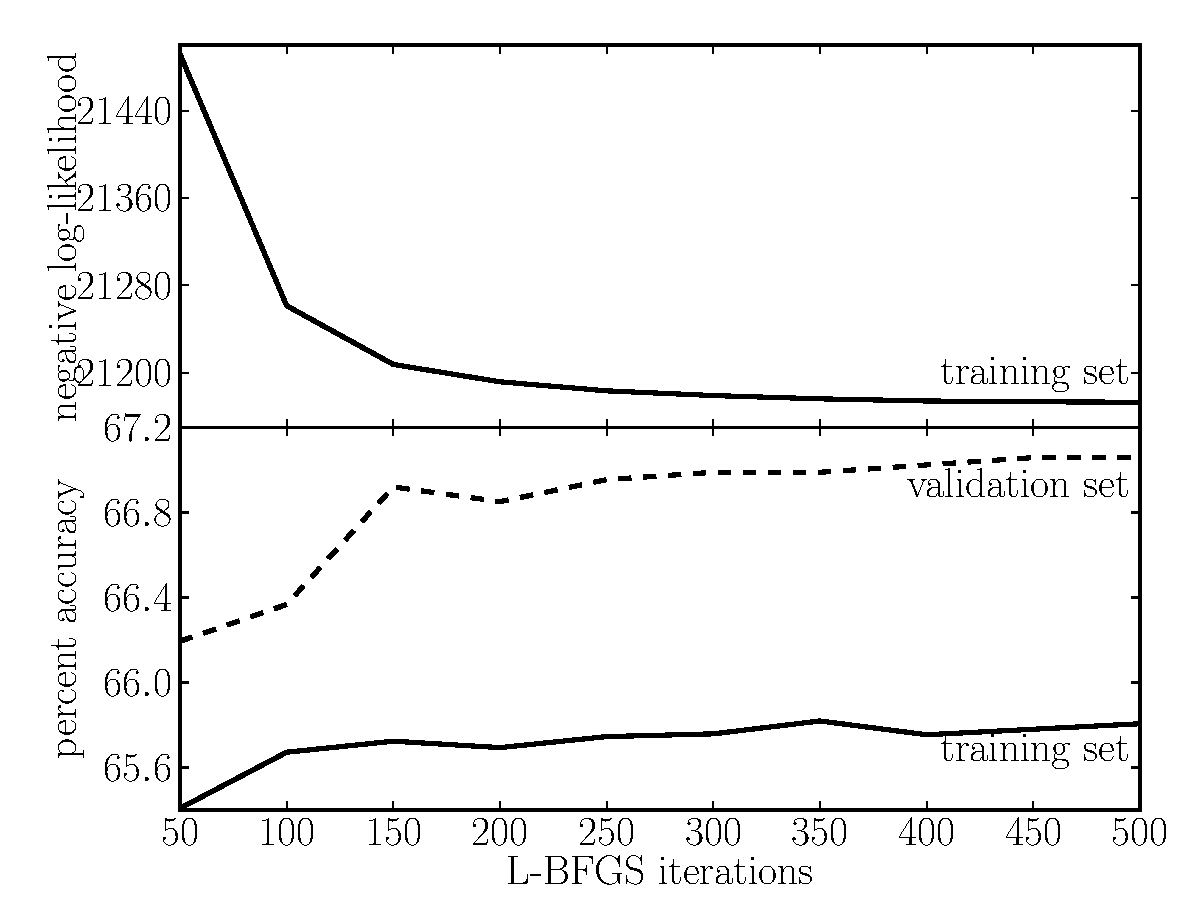
\includegraphics[width=\textwidth]{unigram_convergence.pdf}
\end{center}
\caption{%
\figlabel{unigram-convergence}}
\end{figure}

\begin{figure}[htbp]
\begin{center}
    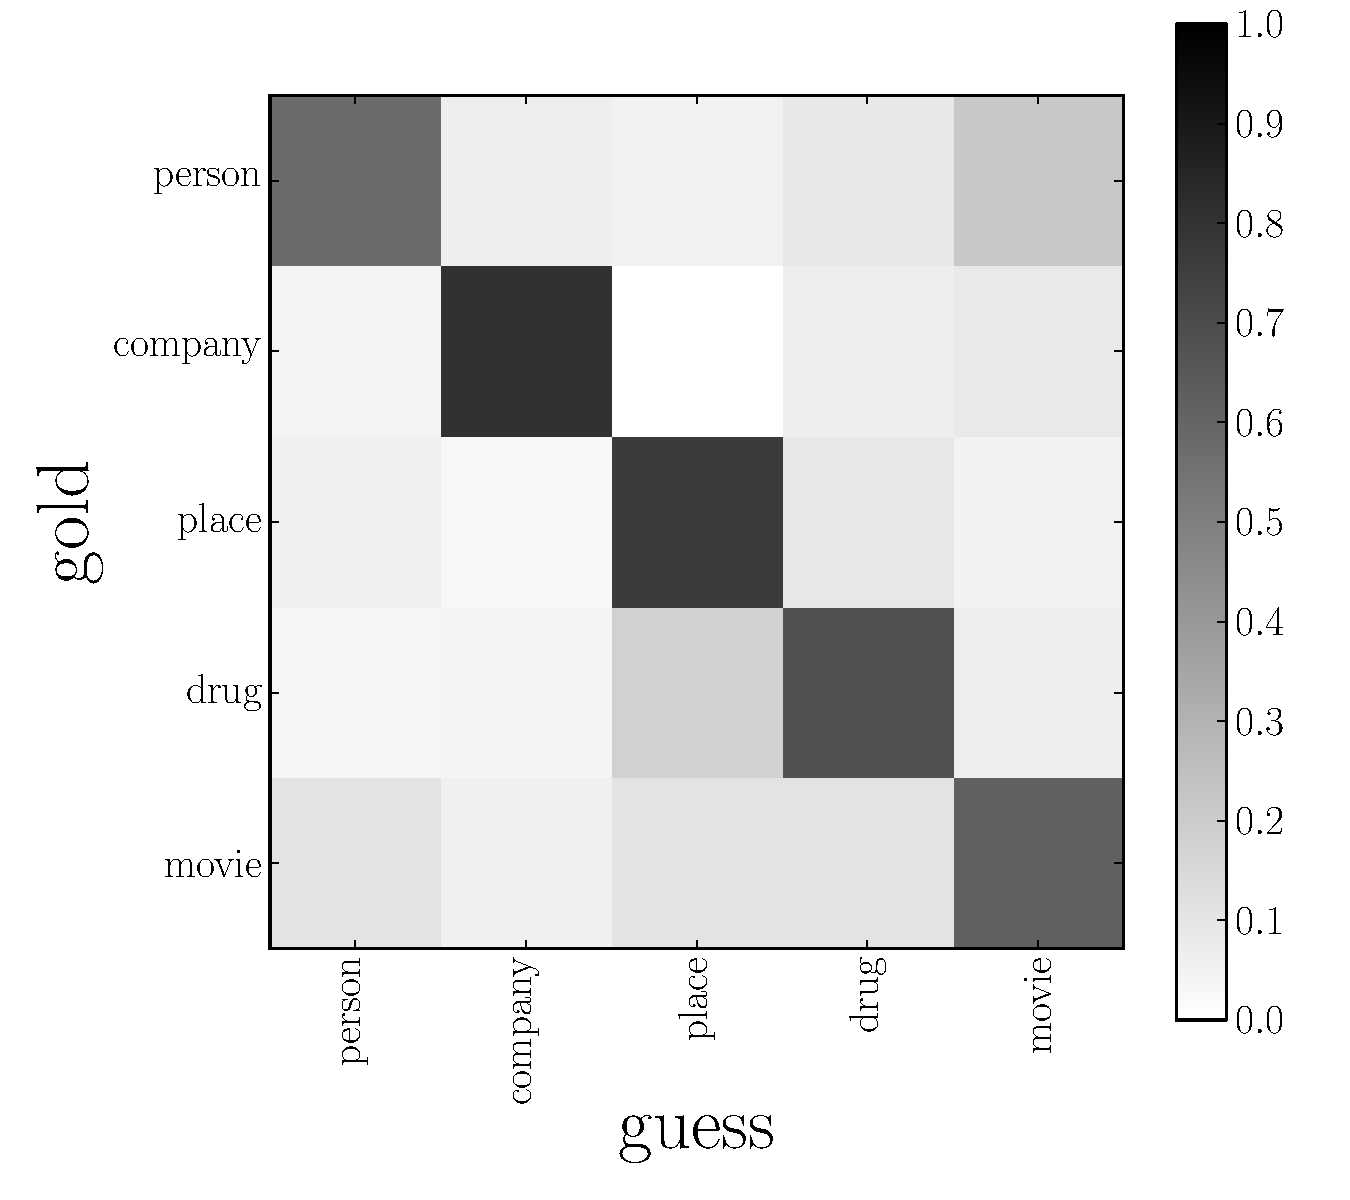
\includegraphics[width=\textwidth]{unigram_confusion.pdf}
\end{center}
\caption{%
\figlabel{unigram-confusion}}
\end{figure}

\begin{figure}[htbp]
\begin{center}
    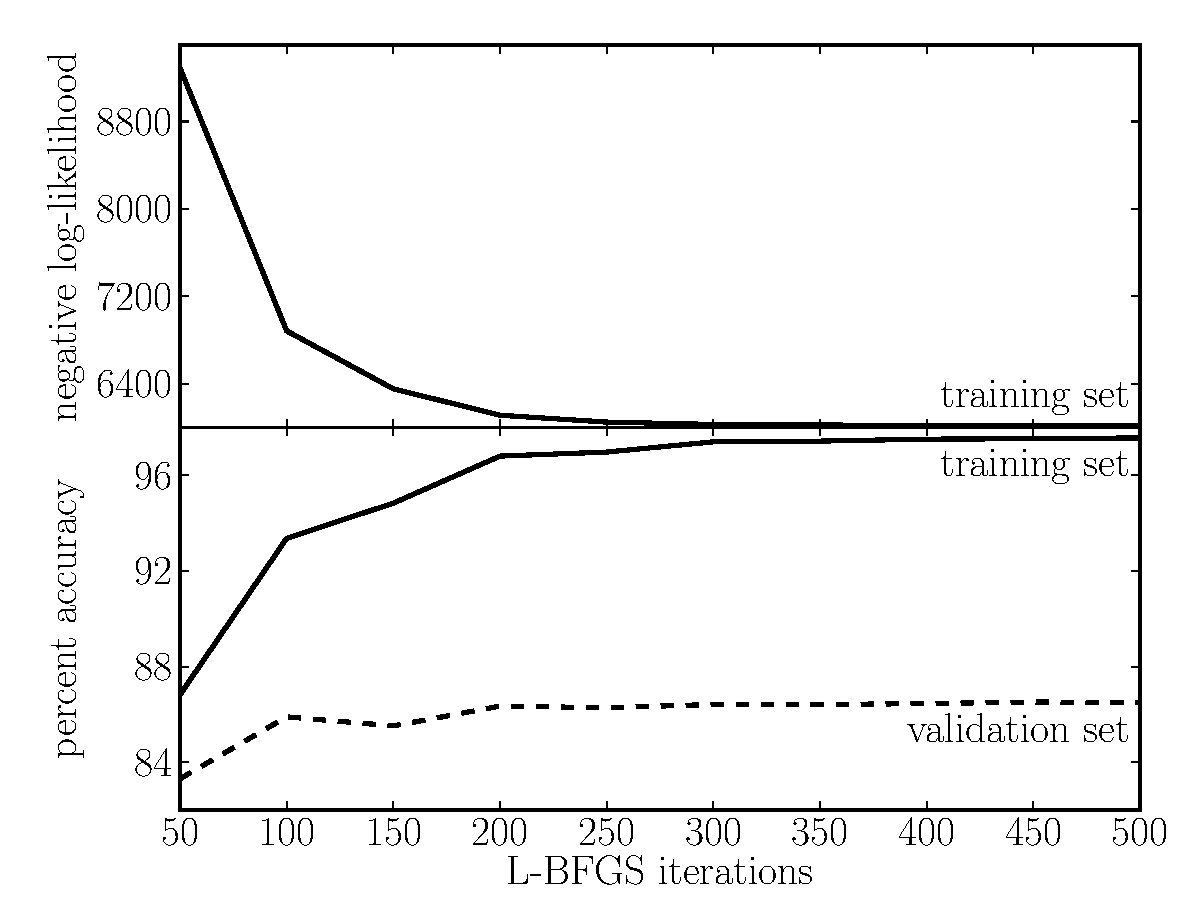
\includegraphics[width=\textwidth]{full_500_convergence.pdf}
\end{center}
\caption{%
\figlabel{full500}}
\end{figure}

\end{document}
